% THIS IS SIGPROC-SP.TEX - VERSION 3.1
% WORKS WITH V3.2SP OF ACM_PROC_ARTICLE-SP.CLS
% APRIL 2009
%
% It is an example file showing how to use the 'acm_proc_article-sp.cls' V3.2SP
% LaTeX2e document class file for Conference Proceedings submissions.
% ----------------------------------------------------------------------------------------------------------------
% This .tex file (and associated .cls V3.2SP) *DOES NOT* produce:
%       1) The Permission Statement
%       2) The Conference (location) Info information
%       3) The Copyright Line with ACM data
%       4) Page numbering
% ---------------------------------------------------------------------------------------------------------------
% It is an example which *does* use the .bib file (from which the .bbl file
% is produced).
% REMEMBER HOWEVER: After having produced the .bbl file,
% and prior to final submission,
% you need to 'insert'  your .bbl file into your source .tex file so as to provide
% ONE 'self-contained' source file.
%
% Questions regarding SIGS should be sent to
% Adrienne Griscti ---> griscti@acm.org
%
% Questions/suggestions regarding the guidelines, .tex and .cls files, etc. to
% Gerald Murray ---> murray@hq.acm.org
%
% For tracking purposes - this is V3.1SP - APRIL 2009

\documentclass{sig-alternate}

\usepackage{url}

\begin{document}
\conferenceinfo{SIGAda'09,} {November 1--5, 2009, St. Petersburg, Florida, USA.} 
\CopyrightYear{2009}
\crdata{978-1-60558-475-1/09/11} 
\title{Use of SPARK in a Resource Constrained Embedded System}

\numberofauthors{3}
\author{
% 1st. author
\alignauthor
Chad Loseby\\
       \affaddr{Vermont Technical College}\\
       \affaddr{Randolph Center, VT}\\
       \email{closeby@vtc.vsc.edu}
% 2nd. author
\alignauthor
Peter Chapin\\
       \affaddr{Vermont Technical College}\\
       \affaddr{Randolph Center, VT}\\
       \email{pchapin@vtc.vsc.edu}
% 3rd. author
\alignauthor
Carl Brandon\\
       \affaddr{Vermont Technical College}\\
       \affaddr{Randolph Center, VT}\\
       \email{cbrandon@vtc.vsc.edu}
}

% \date{30 July 1999}
\maketitle

\begin{abstract}
  We are constructing a remote sensing buoy that will be deployed on the Arctic sea ice north of
  Alaska. The buoy will gather environmental data and transmit that data back to home base via
  the Iridium satellite network. This data will then be used (by others) to refine models of ice
  movement. To enhance reliability the buoy software was written using SPARK Ada. SPARK was also
  helpful in reducing the memory footprint of the software to an acceptable level. Note also
  that the construction of the prototype buoy is a student project. Thus our experience is in an
  educational context.
\end{abstract}

\category{D.2.3}{Software Engineering}{Coding Tools and Techniques}
\category{K.3.2}{Computers and Education}{Computer and Information Science Education}[computer
science education]
\category{C.3}{Special-Purpose and Application-Based Systems}{Real-Time and Embedded Systems}

\terms{Languages, Experimentation}
\keywords{Ada, msp430, spark, student project}

\section{Introduction}

This project is part of a collaboration between Vermont Technical College (VTC) and the
University of Vermont (UVM). Professor Jun Yu, Associate Chair Department of Mathematics \&
Statistics at UVM, has been mathematically modeling the movement of Arctic sea ice as it melts.
This movement is influenced by many factors include temperature, wind speed, and wind direction.
Previous work used satellite photographs of the ice as model input \cite{yu:2005}. However this
work suffered from a lack of ``ground truth'' information.

Vermont Technical College's role in this project is to build several buoys that will be deployed
on the Arctic ice sheet to collect environmental data and transmit that data back to Vermont.
During the 2008-2009 academic year one of us (Loseby) began developing the software for a
prototype buoy as a senior project.

The prototype buoy is built around a CubeSat Kit \cite{www:cubesatkit}. This platform is based
on the TI MSP430 microcontroller. It has significant constraints in processing power, ROM, and
RAM. Specifically our development system used an MSP\-430F149 MCU at 8 MHz with 60 KiB of ROM
and only 2 KiB of RAM. We are interested in using this platform primarily because of its
extremely low power consumption, but also because we have hopes of launching a satellite based
on it as a future project \cite{brandon:2008}. Thus a secondary goal of this project was to gain
experience with this platform.

There are five environmental parameters that the buoy needs to gather. These parameters are
location, temperature, wind speed, and wind direction. Because the ice rotates as it moves it is
also necessary to record a magnetic bearing that, together with location, provides an absolute
orientation of the buoy. These parameters will be gathered once every 30 minutes and transmitted
to home base via a satellite modem using the Iridium short burst data service.

To simplify the design the buoys will be battery powered (instead of solar powered) using a
Tadiran PulsesPlus lithium thionyl chloride 7.2V 19Ah battery. Experience by the Army Cold
Regions Research \& Engineering Laboratory \cite{www:crrel} suggests that this power supply
should be sufficient to run the buoy for up to several months provided care is taken with power
management. Since the buoys are expected to fall into the ocean as the ice melts there is no
need for very long term operation.

Because it will be infeasible to perform any maintenance on the buoy once it is deployed, issues
of reliability are of utmost importance in this application. In particular, a ``crash'' of the
buoy software will cause a failure of the mission. Even worse than an outright crash, however,
would be an error that allows the buoy to operate but return incorrect data. To help avoid these
problems the software was developed using SPARK Ada. The extra level of reliability provided by
SPARK will also be important when we use this platform in a future satellite project.

\section{Software Overview}

The overall structure of the software is rather simple as illustrated by the flowchart in
Figure~\ref{fig:main-loop} The buoy spends most of its time in a deep sleep state. A hardware
timer generates periodic interrupts that are counted by software to accumulate an overall sleep
time of 30 minutes. After being awakened, the buoy collects data from the various sensors,
including time and location information from a GPS unit. This process can take several minutes
but it is done entirely sequentially. The software makes no use of concurrent tasks.

\begin{figure}
\centering
\label{fig:main-loop}
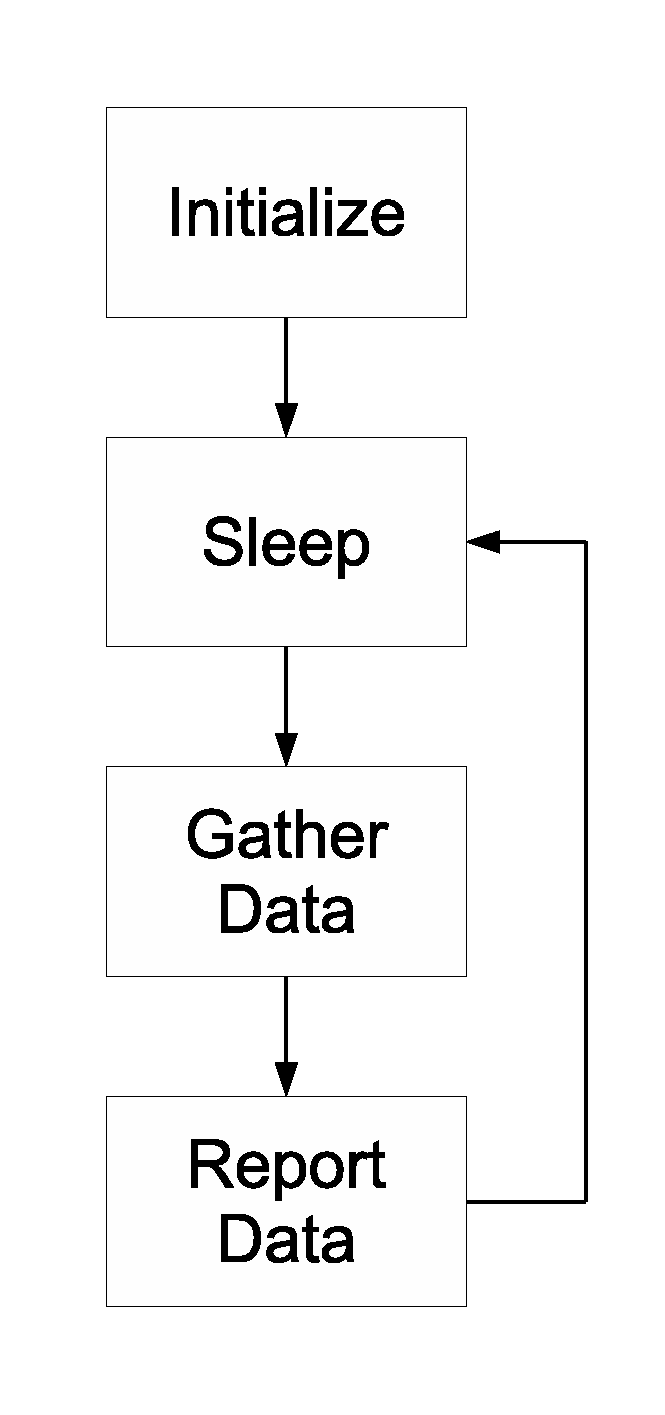
\epsfig{file=Figure-1.eps, height=3in, width=1.5in}
\caption{Buoy software main loop.}
\end{figure}

The gathered data is stored, along with associated time stamps in several buffers with one
buffer for each type of reading. During the reporting phase, the buoy packs as many readings as
possible into a single short burst data packet and transmits that packet to Vermont. It is
possible to pack more data into a short burst data packet than can possibly be gathered in a
single run of the data gathering phase. Thus even if the buffers are non-empty at the start of
a particular loop pass they will eventually drain as the loop executes.

The buffers account for possible problems in either gathering data or reporting it. If a sensor
malfunctions, no data for that sensor will be entered into the buffer but this will not cause
any complications for the handling of other data. If the satellite link goes down, data will
accumulate in the buffers until such time as the link is up again. Note that due to memory
constraints the buffer sizes are small, but because of the low sampling frequency they can still
hold several hours worth of data.

Each buffered data item is time stamped separately. This is because the time at which the data
item is reported may be much later than the time when it was gathered. Since the buoy's location
is one of the data items being reported, the returned (time, location) pairs allow a trajectory
of the buoy to be plotted. This trajectory forms a basis for the interpretation of the other
(time, value) data item pairs.

\section{Tool Chain}

To our knowledge there is no Ada compiler available that specifically targets the MSP430
microcontroller. It may be possible to build a cross compiling version of GNAT using gcc's
MSP430 target \cite{www:mspgcc}. However, this would require specialized knowledge of gcc
technology, which was outside the scope of this project. Instead we used Sofcheck's Ada to C
translator, Ada Magic, to convert our Ada source into plain C \cite{www:adamagic}. We then used
Rowley Associates' CrossWorks C compiler for the MSP430 to generate our final object code
\cite{www:crossworks}. This tool chain is shown in Figure~\ref{fig:tool-chain}. In this figure
the square boxes indicate code and the rounded boxes indicate tools that process the code.

\begin{figure}
\centering
\label{fig:tool-chain}
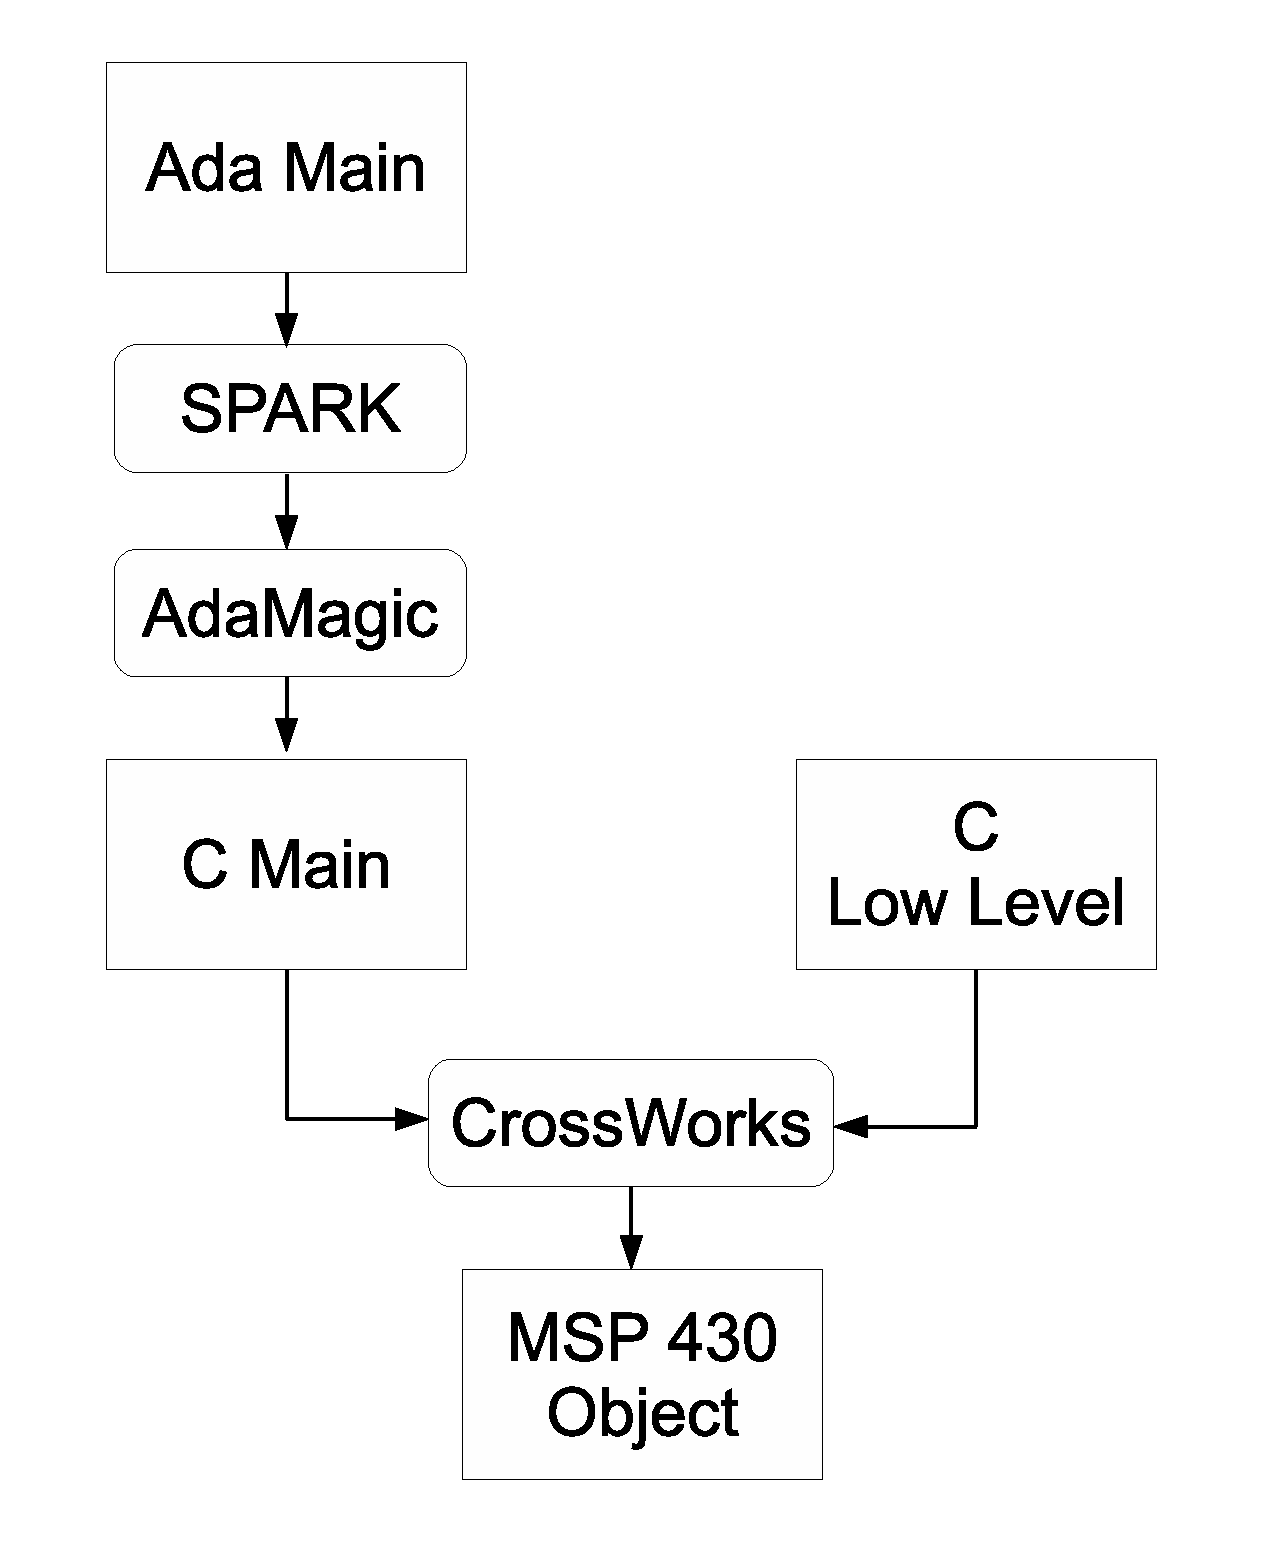
\epsfig{file=Figure-2.eps, height=3.3in, width=2.7in}
\caption{Tool chain.}
\end{figure}

This approach has the advantage of using a back end C compiler that officially supports our
platform. In fact, we used several small C functions for interacting with hardware resources. In
order to keep as much of the code as possible in Ada, and thus visible to the SPARK tools, a
significant effort was made to keep the C functions as simple as possible. For example our
package that exposes the system timer to Ada has the following specification

\begin{verbatim}
package Timer
--# own Timer_Hardware;
is
   procedure Initialize;
   --# global out Timer_Hardware;
   --# derives Timer_Hardware from ;
   pragma Import(C, Initialize);
      
   procedure Sleep;
   --# global in out Timer_Hardware;
   --# derives Timer_Hardware from Timer_Hardware;
   pragma Import(C, Sleep);
end Timer;
\end{verbatim}

Timer\_Hardware is a SPARK own variable that stands for the state of the hardware used by the
timer. We implemented these procedures in C as follows.

\begin{verbatim}
void  Timer_Sleep(void) {
   // Enter Low Power Mode 3
   _BIS_SR(LPM3_bits);
}

void  Timer_Initialize(void) {
   // Timer A: Source TACLK, Clear, Mode 1.
   TACTL = TASSEL0 + TACLR + TAIE; 
   TACTL |= MC1;
  
   // Enable interrupts
   _EINT();
}
\end{verbatim}

We also provided an interrupt service routine for the timer that awakens the processor when the
timer overflows. Procedure Sleep returns when this occurs.

\begin{verbatim}
void Timer_A(void) __interrupt [TIMERA1_VECTOR] 
{
   // If we are overflowing, wake up the system.
   if (TAIV == 10) {
      _BIC_SR_IRQ(LPM3_bits);
   }
}
\end{verbatim}

This C code is necessarily very system specific. However, the Ada code that calls procedures
Initialize and Sleep is free of system dependencies and thus does not require an Ada compiler
with any knowledge of the MSP430 platform. We handled interfacing with other hardware resources
(A/D converters, the serial port, and some LEDs for test purposes) in a similar way.

\section{Comments on SPARK}

Because our platform is extremely resource constrained, we are interested in using the smallest
run time system possible. In fact, we are not using any part of the normal Ada Magic run time
system provided by Sofcheck. In addition to reducing memory, this also simplifies the running
software and enhances reliability by eliminating a large body of code that would otherwise be
outside of SPARK's visibility.

This rather extreme approach was made possible by two factors. First, our system is relatively
simple. The sensors are read one at a time, and the serial communication is all done with polled
I/O. This is acceptable in our case because of the slow time frame in which the system operates.
Most of the software complexity is in formatting and buffering the data, and in gracefully
handling hardware devices that malfunction.

However, our ability to use a minimal run time system is also a direct consequence of our use of
SPARK. For example, SPARK forbids user defined exception handling, so no run time support for
exceptions is needed. The Ada Magic compiler outputs calls to certain run time library functions
for exception handling, but we provided empty implementations of these functions to satisfy the
linker.

SPARK helps us to justify this approach. For example, Ada Magic's output includes calls to a C
function rts\_\-elab\_check that is used to verify that packages are elaborated in an
appropriate order. However, under SPARK rules the semantics of a program are not affected by
elaboration order; the check can never fail. Thus we are justified in providing an empty
implementation for this function.

Ada Magic also emits calls to functions that check for sufficient stack space and for constraint
violations. We are justified in providing empty implementations for these functions only if we
can statically prove that our system will never run out of stack space or raise
Constraint\_Error. Doing this will entail using SPARK proof annotations. At the time of this
writing we have not completed that step, but it is our intention to do so before actually
deploying the buoy.

Notice that there is no danger of accidentally using a run time library function unexpectedly.
Whenever Ada Magic attempts to call a new function from its run time library, our system fails
to link. This forces us to evaluate each new function used. In some cases we changed the Ada
source specifically to avoid using run time library functions we didn't want to implement. For
example in one case Ada Magic called a function to compute the mod operation because C's modulus
operator does not have the right semantics. Rather than provide this function in C, where SPARK
is unable to analyze it, we modified the Ada source so that it was no longer necessary.

The main disadvantage of SPARK was the learning curve associated with it. This was our first
attempt at using SPARK in any capacity and extra time was required to understand the
restrictions imposed by the language as well as how to properly use the annotations.

In addition, debugging the system was complicated by the fact that the CrossWorks debugger had
no knowledge of the original Ada source. All our debugging needed to be done in C which was, in
effect, the assembly language of our system. We are fluent with C and that was very helpful,
even necessary, in a project of this nature.

We also encountered some interesting interactions between SPARK and the Ada Magic compiler. In
one case Ada Magic produced a warning about a possible use of an uninitialized variable.
However, the data flow was such that no uninitialized use was possible. When we included a
spurious initialization of the variable to satisfy Ada Magic, the SPARK Examiner complained that
the initialization had no effect. We eventually decided to disable all warnings from Ada Magic
on the assumption that the SPARK Examiner would be able to detect a superset of the flow
problems detected by Ada Magic.

\section{Educational Opportunities}

Vermont Technical College's mission is education. Thus all of our projects need to be evaluated
in that context. Although Ada is not used as the primary language in any VTC courses, it is
taught at the instructor's discretion as a supplementary language in several courses. Loseby was
first exposed to Ada in a programming languages course taught by Chapin. In addition Ada has
been used for the last two years in a sophomore projects course. None of these courses currently
discuss SPARK; this is the first time anyone at VTC, instructors and students alike, has
attempted to use SPARK in any capacity.

From a student perspective, SPARK was a welcome introduction to static code analysis. Loseby
found the SPARK annotations much easier to understand and write after grasping the concept that
hardware states could be represented and described by those annotations. In many cases, the
process of visualizing the desired behavior in order to write an annotation revealed logical
errors or prompted the refactoring of the code to improve efficiency or maintainability.

Chapin and Brandon intend to build on the experience of this project by using the same approach
in the construction of the software for a VTC satellite. This will be done as one or more senior
projects with the first project group anticipated in the 2009-2010 academic year. In addition
Chapin intends to comment explicitly on SPARK during his fall 2009 delivery of the programming
languages course, using examples taken from this project.

\section{Status and Future Directions}

The work reported here has been on the construction of a single prototype buoy to demonstrate
the feasibility of our design and of our approach. At the time of this writing the development
of the prototype is still in progress. We have demonstrated reading temperature and wind
direction data, and sending that data back to Vermont via the Iridium network. However, we still
need to implement support for gathering and transmitting wind speed and magnetometer data.

In addition we are currently only using SPARK data flow annotations. While this has been helpful
with finding bugs in our software, we still need to make use of the SPARK proof tools to show
that certain exceptions can't occur. Our system depends on this because of the way we have
eliminated exception handling support in the run time system.

Funding to construct the prototype continues through the end of this year and we anticipate
completing the prototype in time to conduct field tests during the northern hemisphere 2009-2010
winter season. In the long term we hope to receive funding to manufacture ten to twenty buoys
for deployment in the Arctic perhaps in March of 2011.

\section{Conclusions}

Using SPARK Ada in an educational setting to develop software for a highly constrained embedded
system without a native Ada compiler is feasible. Although there are some aspects of our project
that have yet to be completed, we are confident that we will be able to build on the success we
have had so far. One interesting benefit of using SPARK was the way it allowed us to
eliminate significant amounts of run time support. This was essential in our case due to the
very limited amounts of memory available to us.

\vfill\eject
\section{Acknowledgments}

This project is supported by grants from the Vermont Space Grant Consortium, a part of the NASA
Space Grant program. Vermont Technical College also received generous donations of commercial
software from AdaCore, SofCheck, Praxis, and Rowley Associates.

%
% The following two commands are all you need in the initial runs of your .tex file to produce
% the bibliography for the citations in your paper.
\bibliographystyle{abbrv}
\bibliography{../../../LaTeX/CubeSat}
%% sigproc.bib is the name of the Bibliography in this case. You must have a proper ".bib" file
%% and remember to run:
%%   latex bibtex latex latex
%% to resolve all references
%%
%% ACM needs 'a single self-contained file'!
%%
%%APPENDICES are optional
%%\balancecolumns
%\appendix
%\section{References}
%Generated by bibtex from your ~.bib file. Run latex, then bibtex, then latex twice (to resolve
%references) to create the ~.bbl file. Insert that ~.bbl file into the .tex source file and
%comment out the command \texttt{{\char'134}thebibliography}.

\balancecolumns

\end{document}
